\documentclass[12pt]{article}
\usepackage{charter} % font
\usepackage[margin=1in]{geometry} % margin
\usepackage{varioref}
\usepackage{hyperref} % hyperlinks
\usepackage{enumitem} % Enumeration
\graphicspath{ {.} } % images

\usepackage[lined,dotocloa]{algorithm2e} % Pseudocode
\labelformat{algocf}{\textit{alg.}\,(#1)}


%%%%%%%%%%%%%%%%%%%%%%%%%%%%%%%%%%%%%%%%%%%%%%%%%%%%%%%%%%%%%%%%%%%%%%%%%%%%%%%%

\title{%
	\textbf{Assignment 3 \\ 
	Sorting: Putting your affairs in order \\
	\large WRITEUP} }

	\author{Zack Traczyk \\ CSE13S - Spring 2021}
	\date{Due: April 25\textsuperscript{th} at 11:59 pm}

%%%%%%%%%%%%%%%%%%%%%%%%%%%%%%%%%%%%%%%%%%%%%%%%%%%%%%%%%%%%%%%%%%%%%%%%%%%%%%%%

	\begin{document}

	\maketitle

	\section{Time Complexity}
	
	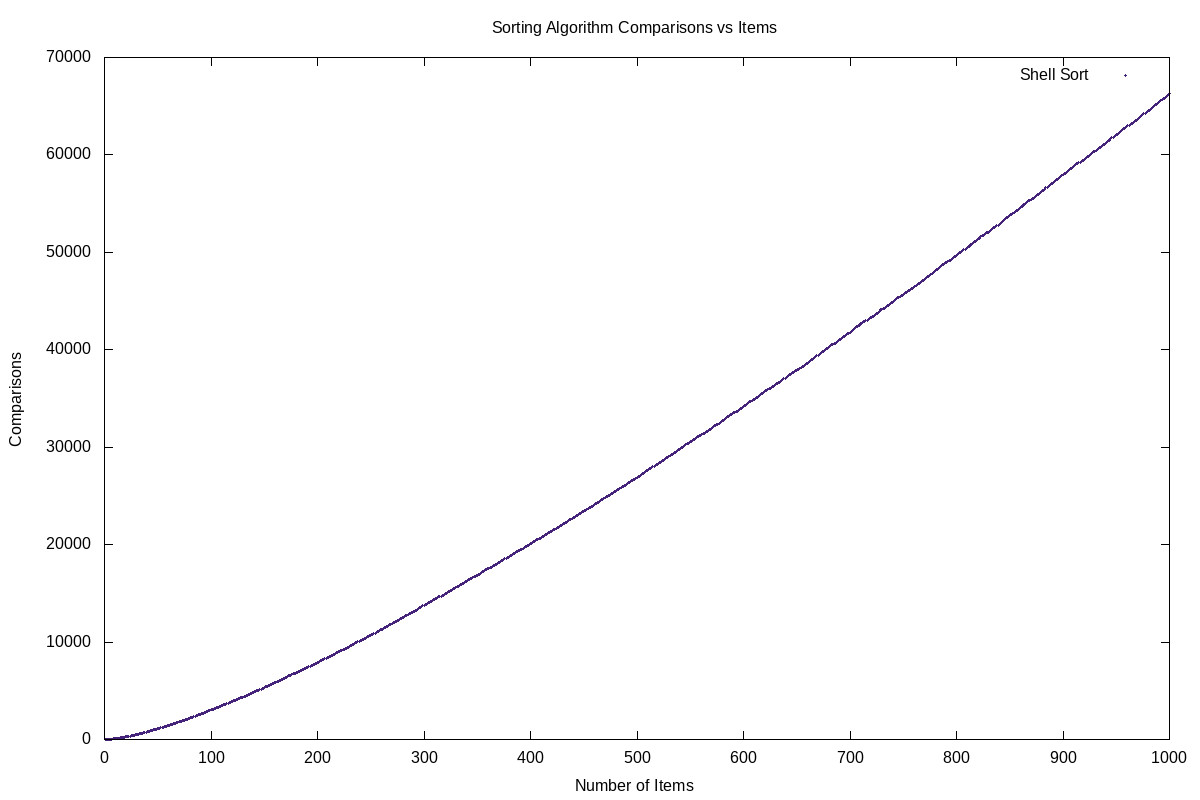
\includegraphics{shell}

	\subsection{Reverse Order}

	\subsection{Small Number of Elements}

	\subsection{Large Number of Elements}

	\section{What i learend}

	\section{how i experimented}

	\section{Size of Stack and Queue in relation to input}

	\end{document}

